\label{section:2d_hillslope_example}
These two examples compare 2D variably-saturated flow in a hillslope:
\begin{description}
    \item [Example 1 (\texttt{2\_VSF\_Hillslope}):] A \gwf\ domain  simultaneously receives recharge to and allows drainage from it's top layer of cells.
    \item [Example 2 (\texttt{4\_SWF\_RCH\_CRD}):] A fully-coupled \gwf-\swf\ system receives recharge to the \swf\ domain and allows drainage from the \swf\ cell located at the downstream outflow boundary.
\end{description}

The following parameter values were used for the \gwf\ domain in both examples:

\begin{center}
    \begin{tabular}{lll}  \hline
        Parameter                             & Value & Unit                                \\ \hline
        Specific yield (porosity)             &  0.1                        &               \\
        Hydraulic conductivity                &  31.536    &   m yr$^{-1}$  \\
        Specific storage coefficient          &  $ 1 \times 10^{-7}$        &   m$^{-1}$    \\
        Van Genuchten Alpha         &  $3.34 \times 10^{-2}$                        &   m$^{-1}$    \\
        Van Genuchten Beta          &  1.982                          &               \\
        Residual saturation                   &  0.2771                        &               \\
    \hline
    \end{tabular}
\end{center}

The Van Genuchten unsaturated function type was used.

For the \swf\ domain of example 2, the following parameter values were used:

\begin{center}
    \begin{tabular}{lll}  \hline
        Parameter                           & Value                     &   Unit            \\ \hline
        Manning's coefficient               &  $1.7 \times 10^{-9}$     &   yr m$^{-1/3}$   \\
        Depression storage height           &  $1 \times 10^{-6}$       &   m               \\
        Obstruction storage height          &  $1 \times 10^{-6}$       &   m               \\
        Depth for smoothing height 1        &  $1 \times 10^{-6}$       &   m               \\
        Depth for smoothing height 2        &  $1 \times 10^{-6}$       &   m               \\
    \hline
    \end{tabular}
\end{center}

An initial head of 0.0 m was assigned to the \gwf\ domain in both examples.

For example 1, a recharge flux of 0.5 m/yr was applied to the entire top of the \gwf\ domain.  The drain boundary condition applied to the top layer of \gwf\ cells was assigned a drain elevation equal to the ground surface elevation and a drain conductance of 1000 m/yr.

For example 2, an initial surface water depth of $1 \times 10^{-3}$ m was assigned to the \swf\ domain.  A recharge flux of 0.5 m/yr was applied to the entire \swf\ domain. A critical depth boundary condition was assigned to the \swf\ cell located at the downstream outflow boundary.

The simulation was run for 1000 years during which time steady-state conditions were achieved.

\pagebreak
Here is a comparison of hydraulic head  at steady-state for examples 1 (upper plot) and 2 (lower plot):

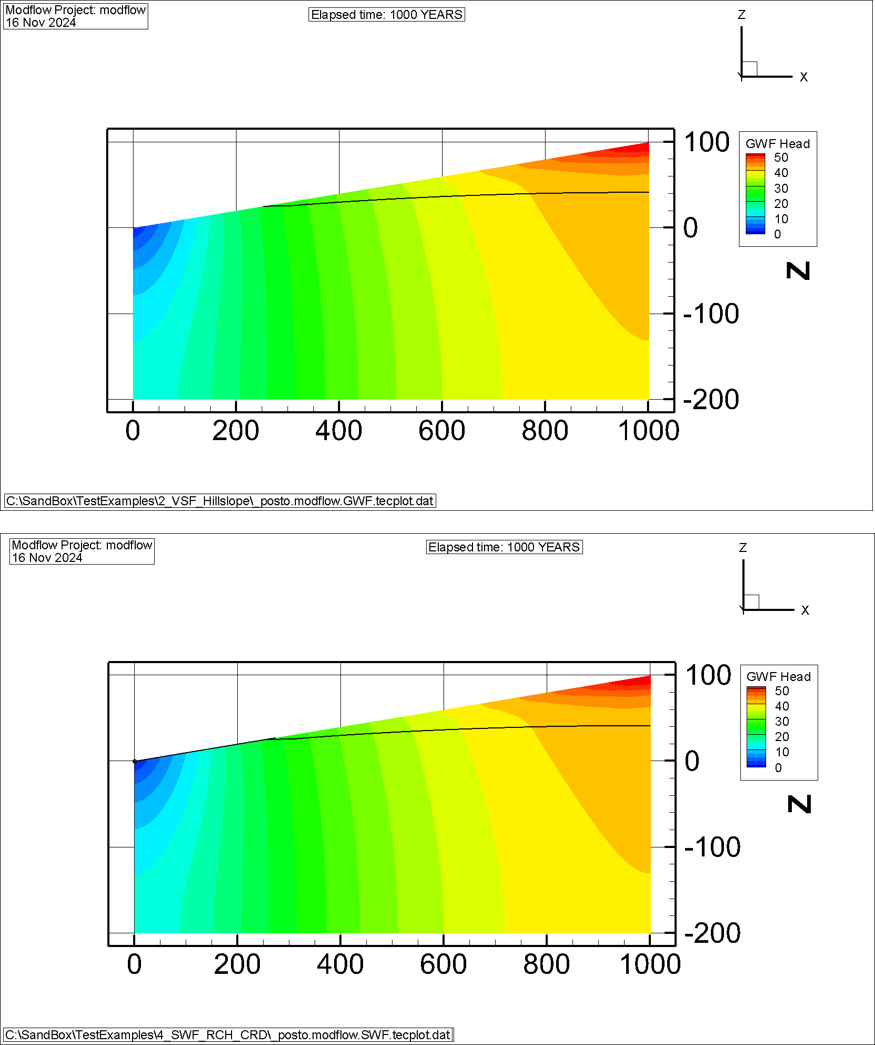
\includegraphics[width=0.87\textwidth]{5_5_Head_WaterTableComparison}

The results are similar for both examples. The water table is shown as a heavy black line.  In the lower plot, the black line extends into the \swf\ domain and represents surface water depths greater than $7.7 \times 10^{-6}$ m.  The critical depth boundary condition that was assigned to the \swf\ cell located at the downstream outflow boundary is indicated by the small black sphere.

\pagebreak
Here is a comparison of volumetric flow rates versus time  for examples 1 (upper plot) and 2 (lower plot):

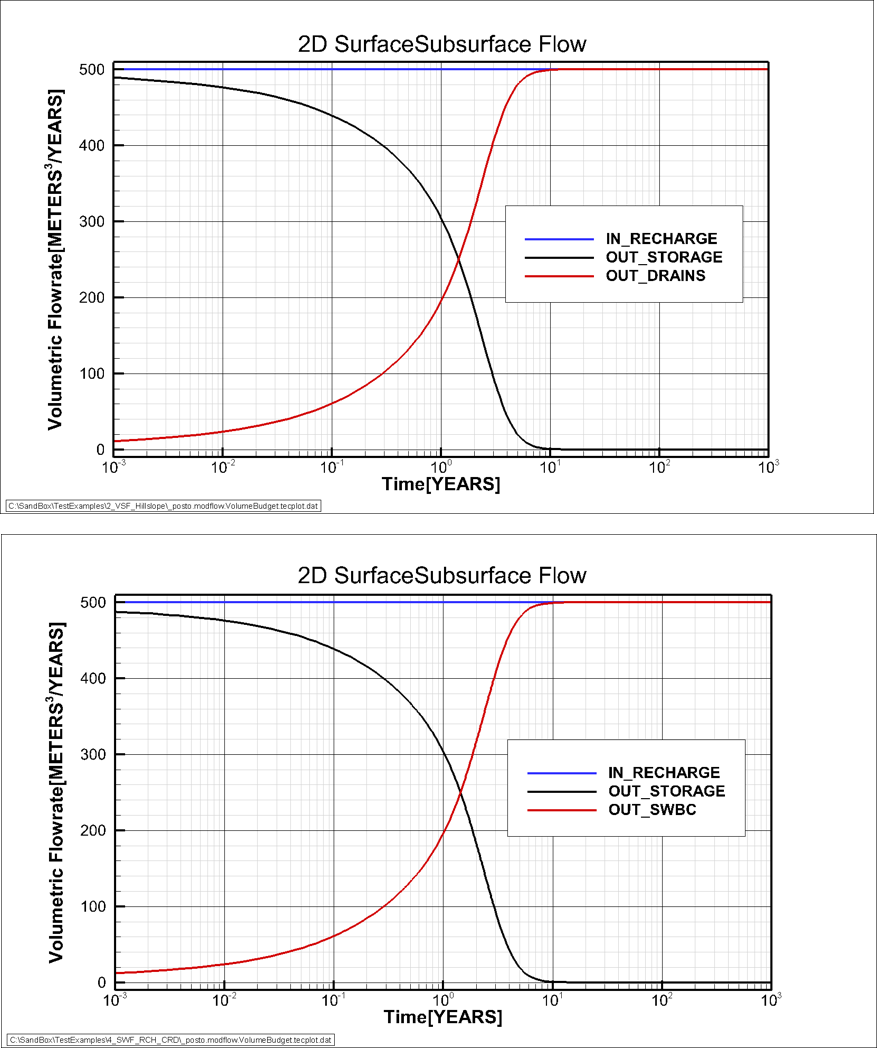
\includegraphics[width=0.87\textwidth]{5_6_WaterBudgetComparison}

The results are essentially identical for both examples, showing that the critical depth boundary outflow ({\sf OUT\_SWBC}) is being calculated correctly. In both examples, water coming out of storage in the \gwf\ domain is balanced by discharge along the top (example 1)  or at the downstream outflow boundary (example 2).

